\documentclass[11pt]{scrartcl}

\usepackage{cancel}
\usepackage[utf8]{inputenc}
\usepackage{mathtools}
\usepackage[sexy]{evan}

\title{19EGMO2}
\author{Himadri Mandal}

\begin{document}
\maketitle

\section{Solution}
\begin{soln}
	
\raggedright
The answer is $\frac{n(n+1)}{2}$. 

\begin{claim}{Construction}
\end{claim}
\begin{proof}
Consider this easily generalisable construction: (credits to @vEnhance for image) 
\begin{center}
	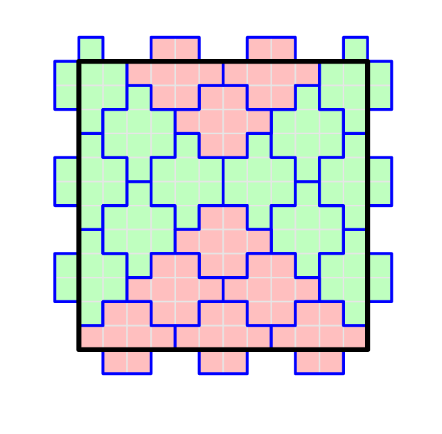
\includegraphics[scale=0.3]{19EGMO2.jpg}
\end{center}
\end{proof}
Call the cells adjacent to a domino its \textbf{\color{red}cloak}. Note that a domino's cloak might have $\{5,6,7,8\}$ cells, let there be $a$ cells with cloak $5$, $b$ with $6$, $c$ with $7$ and $d$ with $8$.

We have $5a+6b+7c+8d = 4n^2$.

\begin{claim}
$$4a+4b+3c \leq 4(2n-1)$$
\end{claim}
\begin{proof}
	Pretty straight forward, cells with cloak $5$ cover $4$, $6$ cover $4$ and $7$ cover $5$, cells with cloak $8$ \textit{don't} lie on the border.
\end{proof}

To finish, 

$$4n^2 + 2(2n-1) \geq (5a+6b+7c+8k) + \frac12(4a+4b+3c)$$
$$= 8\cycsum(a) + \frac12 c - a \geq 8 \cycsum a - 4 \implies \cycsum(a) \leq \frac{n(n+1)}{2} + \frac14$$


\end{soln}
\end{document}
